\clearpage
\section{Dasar Teori}
\subsection{\textit{Supervised Learning} dan Klasifikasi}
\textit{Supervised learning} adalah paradigma pembelajaran mesin yang mempelajari fungsi pemetaan $h:\mathcal{X}\rightarrow\mathcal{Y}$ dari kumpulan contoh berlabel $D=\{(\mathbf{x}_i,y_i)\}_{i=1}^{n}$. Setiap $\mathbf{x}_i$ adalah vektor fitur, sedangkan $y_i$ adalah keluaran yang diketahui. Apabila $\mathcal{Y}$ berupa himpunan kelas berhingga, persoalannya disebut klasifikasi. Pada tugas ini $\mathcal{Y}=\{0,1\}$ sehingga persoalannya merupakan klasifikasi biner.

Tujuan pembelajaran bukan menghafal data latih, melainkan memperoleh hipotesis yang menggeneralisasi dengan baik pada data yang belum pernah dilihat. Hipotesis yang terlalu sederhana menghasilkan \textit{underfitting}, yaitu galat besar pada data latih maupun data baru. Sebaliknya, hipotesis yang terlalu kompleks dapat mengikuti derau pada data latih sehingga mengalami \textit{overfitting}. Oleh sebab itu, kinerja model selalu diukur pada data yang terpisah dari data latih, dan kompleksitas model dikendalikan melalui \textit{hyperparameter}, regularisasi, atau pemangkasan.

Sebagian besar model pada tugas ini menghasilkan skor peluang $\hat{p}(\mathbf{x})=P(y=1\mid\mathbf{x})$. Label diperoleh dengan membandingkan skor tersebut terhadap ambang $\tau$, yaitu $\hat{y}=\mathbb{1}[\hat{p}(\mathbf{x})\geq\tau]$. Ambang baku adalah $\tau=0{,}5$, tetapi ambang dapat diubah ketika biaya kesalahan tidak simetris, sebagaimana dibahas pada Subbab~\ref{sec:teori-cost}.

\subsection{CRISP-DM, \textit{Data Understanding}, dan \textit{Data Preparation}}
\textit{Cross-Industry Standard Process for Data Mining} (CRISP-DM) membagi proyek data menjadi enam fase: \textit{business understanding}, \textit{data understanding}, \textit{data preparation}, \textit{modeling}, \textit{evaluation}, dan \textit{deployment}. Fase-fase tersebut bersifat iteratif. Temuan pada pemodelan sering memaksa kembali ke tahap persiapan data. Templat notebook tugas ini mengikuti urutan yang sama, mulai dari pemahaman data hingga pengumpulan prediksi.

\textit{Data understanding} mencakup deskripsi data (ukuran, tipe, dan arti kolom), eksplorasi (distribusi dan hubungan fitur dengan target), serta verifikasi kualitas (nilai hilang, duplikat, nilai tidak valid, dan pencilan). Hasil fase ini menentukan langkah persiapan yang diperlukan.

\textit{Data preparation} mengubah data mentah menjadi representasi yang dapat diproses algoritma. Langkah utamanya adalah sebagai berikut.
\begin{enumerate}
    \setlength{\itemsep}{0pt}
    \item \textbf{\textit{Data cleaning}}\\
    Nilai hilang dapat dihapus atau diimputasi, misalnya dengan median untuk fitur numerik dan modus untuk fitur kategorikal. Median lebih tahan terhadap pencilan daripada rata-rata. Baris duplikat dan baris yang melanggar aturan domain juga ditangani pada tahap ini. Pencilan dapat dideteksi dengan aturan IQR, yaitu nilai di luar $[Q_1-1{,}5\,\mathrm{IQR},\,Q_3+1{,}5\,\mathrm{IQR}]$, lalu dipotong (\textit{clipping}) ke persentil tertentu.
    \item \textbf{\textit{Data transformation}}\\
    Fitur kategorikal diubah menjadi angka melalui \textit{one-hot encoding}, yaitu satu kolom biner untuk setiap kategori. Fitur numerik diskalakan agar setara, misalnya dengan standardisasi $z=(x-\mu)/\sigma$ atau normalisasi min-max $x'=(x-x_{\min})/(x_{\max}-x_{\min})$. Penskalaan penting bagi model berbasis jarak dan gradien, karena fitur bernilai besar akan mendominasi jarak maupun langkah optimasi.
    \item \textbf{\textit{Feature construction} dan \textit{feature selection}}\\
    Fitur turunan dapat merangkum beberapa kolom menjadi informasi yang lebih bermakna. Pemilihan fitur membuang atribut yang kurang relevan. Salah satu ukurannya adalah \textit{mutual information} $I(X;Y)=\sum_{x,y}p(x,y)\log_2\frac{p(x,y)}{p(x)p(y)}$, yang bernilai nol apabila fitur dan target saling bebas.
    \item \textbf{\textit{Dimensionality reduction}}\\
    \textit{Principal Component Analysis} (PCA) memproyeksikan data ke arah vektor eigen matriks kovarians dengan ragam terbesar. Jumlah komponen dipilih agar proporsi ragam kumulatif melewati batas tertentu, misalnya 95\%.
    \item \textbf{Penanganan ketidakseimbangan kelas}\\
    \textit{Random oversampling} menyalin sampel kelas minoritas secara acak hingga jumlah kedua kelas seimbang. Teknik ini hanya boleh diterapkan pada data latih.
\end{enumerate}

Prinsip terpenting dalam persiapan data adalah mencegah \textit{data leakage}. Seluruh statistik yang dipelajari dari data, seperti median imputasi, batas \textit{clipping}, kategori \textit{encoder}, rata-rata dan simpangan baku \textit{scaler}, skor seleksi fitur, serta komponen PCA, harus di-\textit{fit} hanya pada data latih. Data validasi dan data uji cukup di-\textit{transform}. Jika aturan ini dilanggar, skor validasi menjadi terlalu optimis dan tidak mencerminkan kinerja pada data baru.

\subsection{\textit{k-Nearest Neighbors}}
\textit{k-Nearest Neighbors} (KNN) adalah metode \textit{instance-based} atau \textit{lazy learning}. Pada fase pelatihan, KNN hanya menyimpan seluruh data latih. Ketika menerima titik kueri $\mathbf{x}_q$, KNN menghitung jarak ke setiap data latih, mengambil $k$ tetangga terdekat $N_k(\mathbf{x}_q)$, lalu menentukan kelas berdasarkan suara tetangga tersebut. Gambar~\ref{fig:teori-knn} mengilustrasikan proses ini.

Jarak yang umum digunakan adalah keluarga Minkowski orde $p$:
\begin{equation}
    d_p(\mathbf{a},\mathbf{b})=\left(\sum_{j=1}^{m}|a_j-b_j|^{p}\right)^{1/p}.
    \label{eq:minkowski}
\end{equation}
Nilai $p=1$ menghasilkan jarak Manhattan, sedangkan $p=2$ menghasilkan jarak Euclidean. Untuk klasifikasi biner, peluang kelas positif diperkirakan dari proporsi tetangga positif. Dengan pembobotan jarak, tetangga yang lebih dekat diberi pengaruh lebih besar:
\begin{equation}
    \hat{p}(\mathbf{x}_q)=\frac{\sum_{i\in N_k(\mathbf{x}_q)}w_i\,y_i}{\sum_{i\in N_k(\mathbf{x}_q)}w_i},\qquad
    w_i=\begin{cases}1 & \text{(\textit{uniform})},\\ 1/d(\mathbf{x}_q,\mathbf{x}_i) & \text{(\textit{distance})}.\end{cases}
    \label{eq:knn-proba}
\end{equation}

Nilai $k$ mengatur keseimbangan bias dan variansi. Nilai $k$ kecil membuat batas keputusan sangat lokal dan peka derau, sedangkan nilai $k$ besar menghaluskan batas keputusan tetapi dapat mengaburkan pola lokal. Karena seluruh perhitungan terjadi saat prediksi, kompleksitas waktu prediksi naif adalah $O(n\,m)$ untuk setiap kueri, dengan $n$ jumlah data latih dan $m$ jumlah fitur. KNN juga sangat bergantung pada skala fitur dan rentan terhadap \textit{curse of dimensionality}, yaitu kondisi ketika jarak antartitik menjadi kurang informatif pada dimensi tinggi.

\begin{figure}[htbp]
    \centering
    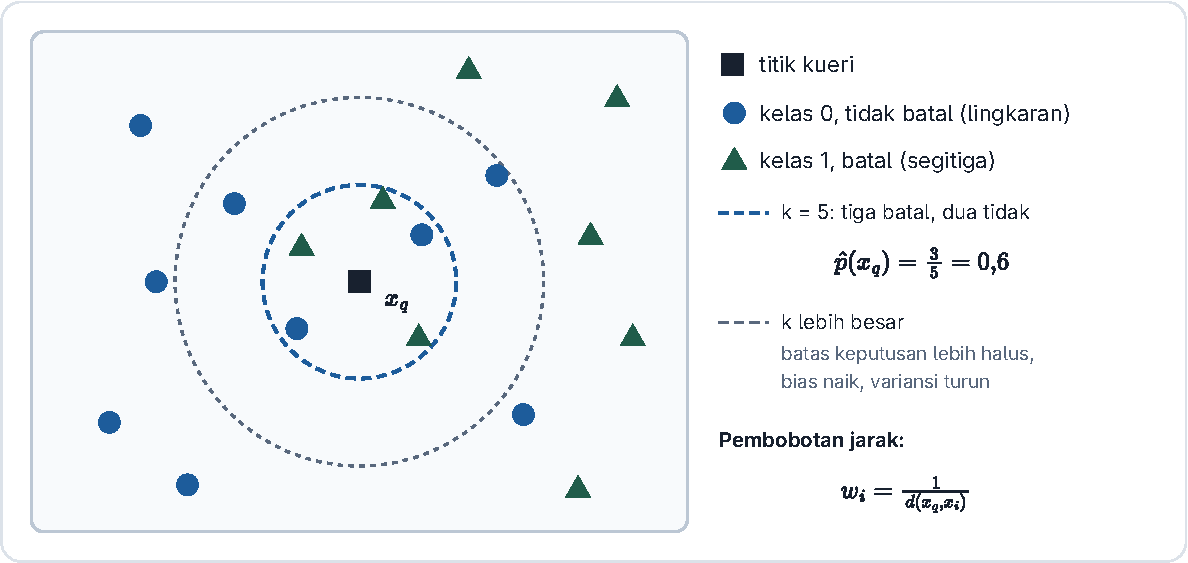
\includegraphics[width=0.82\textwidth]{diagram/knn.pdf}
    \caption{Ilustrasi KNN: kelas titik kueri ditentukan oleh $k$ tetangga terdekat. Jari-jari lingkaran bergantung pada nilai $k$.}
    \label{fig:teori-knn}
\end{figure}

\subsection{\textit{Decision Tree Learning}}
\textit{Decision Tree Learning} (DTL) membangun pohon keputusan secara \textit{top-down} dan rakus (\textit{greedy}). Setiap simpul internal menguji satu atribut, setiap cabang mewakili hasil uji, dan setiap daun menyimpan distribusi kelas. Algoritma dasar ID3 memilih atribut yang paling memurnikan data pada setiap simpul, lalu mengulang proses secara rekursif pada setiap cabang hingga data murni atau atribut habis.

\subsubsection{Entropi, \textit{Information Gain}, dan \textit{Gain Ratio}}
Ketidakmurnian himpunan $S$ diukur dengan entropi
\begin{equation}
    H(S)=-\sum_{c}p_c\log_2 p_c,
    \label{eq:entropy}
\end{equation}
dengan $p_c$ proporsi kelas $c$ pada $S$. Entropi bernilai nol untuk himpunan murni dan bernilai maksimum satu bit untuk dua kelas yang seimbang. Pengurangan entropi setelah memecah $S$ menurut atribut $A$ disebut \textit{information gain}:
\begin{equation}
    \mathrm{Gain}(S,A)=H(S)-\sum_{v\in\mathrm{Values}(A)}\frac{|S_v|}{|S|}H(S_v).
    \label{eq:gain}
\end{equation}
\textit{Information gain} cenderung memilih atribut dengan banyak nilai, karena atribut seperti itu memecah data menjadi banyak subset kecil yang mudah murni. C4.5 mengoreksi bias tersebut dengan \textit{gain ratio}:
\begin{equation}
    \mathrm{SplitInfo}(S,A)=-\sum_{v}\frac{|S_v|}{|S|}\log_2\frac{|S_v|}{|S|},\qquad
    \mathrm{GainRatio}(S,A)=\frac{\mathrm{Gain}(S,A)}{\mathrm{SplitInfo}(S,A)}.
    \label{eq:gain-ratio}
\end{equation}
Karena \textit{gain ratio} dapat membesar secara semu ketika $\mathrm{SplitInfo}$ mendekati nol, C4.5 hanya membandingkan \textit{gain ratio} di antara atribut yang \textit{information gain}-nya minimal sebesar rata-rata \textit{gain} seluruh kandidat.

\begin{contoh}
Sebagai ilustrasi, himpunan $S$ berisi 10 pemesanan: 4 batal dan 6 tidak batal, sehingga $H(S)=-(0{,}4\log_2 0{,}4+0{,}6\log_2 0{,}6)=0{,}9710$. Atribut biner $A$ memecah $S$ menjadi dua cabang berisi 5 sampel. Cabang pertama memuat 4 batal dan 1 tidak batal dengan $H=0{,}7219$, sedangkan cabang kedua murni tidak batal dengan $H=0$. Dengan demikian,
\[
\mathrm{Gain}(S,A)=0{,}9710-\tfrac{5}{10}(0{,}7219)-\tfrac{5}{10}(0)=0{,}6100,\qquad \mathrm{SplitInfo}(S,A)=1,
\]
sehingga $\mathrm{GainRatio}(S,A)=0{,}6100$. Karena pemecahannya seimbang, \textit{split information} bernilai satu dan \textit{gain ratio} sama dengan \textit{gain}. Atribut yang memecah data menjadi banyak cabang kecil akan memiliki \textit{split information} lebih besar dan karenanya dihukum.
\end{contoh}

CART memakai ukuran lain, yaitu indeks Gini $G(S)=1-\sum_c p_c^2$, dan selalu membentuk pohon biner. Tabel~\ref{tab:varian-dtl} merangkum perbedaan ketiga varian tersebut.

\begin{table}[htbp]
    \centering
    \small
    \renewcommand{\arraystretch}{1.15}
    \begin{tabularx}{\textwidth}{@{}lXXX@{}}
        \toprule
        Aspek & ID3 & C4.5 & CART \\
        \midrule
        Ukuran pemisahan & \textit{Information gain} & \textit{Gain ratio} & Indeks Gini \\
        Atribut numerik & Tidak langsung & Ambang biner $A\leq t$ & Ambang biner $A\leq t$ \\
        Atribut kategorikal & Cabang per nilai & Cabang per nilai & Pemisahan biner himpunan nilai \\
        Nilai hilang & Tidak ditangani & Bobot pecahan & \textit{Surrogate split} \\
        Pemangkasan & Tidak ada & \textit{Error-based pruning} & \textit{Cost-complexity pruning} \\
        \bottomrule
    \end{tabularx}
    \caption{Perbandingan varian DTL.}
    \label{tab:varian-dtl}
\end{table}

\subsubsection{Atribut Kontinu dan Nilai Hilang}
Atribut kontinu ditangani dengan mencari ambang $t$ sehingga data terbagi menjadi $A\leq t$ dan $A>t$. Kandidat ambang cukup diambil dari titik tengah dua nilai berurutan yang berbeda setelah data diurutkan, karena ambang optimum untuk ukuran berbasis entropi selalu berada di antara dua nilai seperti itu.

Untuk nilai hilang, C4.5 menghitung \textit{gain} hanya pada sampel yang nilainya diketahui, lalu mengalikannya dengan proporsi sampel yang diketahui. Saat pemecahan, sampel dengan nilai hilang dikirim ke semua cabang dengan bobot pecahan sebanding dengan proporsi sampel diketahui pada cabang tersebut. Saat prediksi, data uji yang nilainya hilang menelusuri seluruh cabang, dan distribusi kelas dari daun-daun yang dicapai digabung sesuai bobot cabangnya. Gambar~\ref{fig:teori-dtree} memperlihatkan mekanisme ini.

\begin{figure}[htbp]
    \centering
    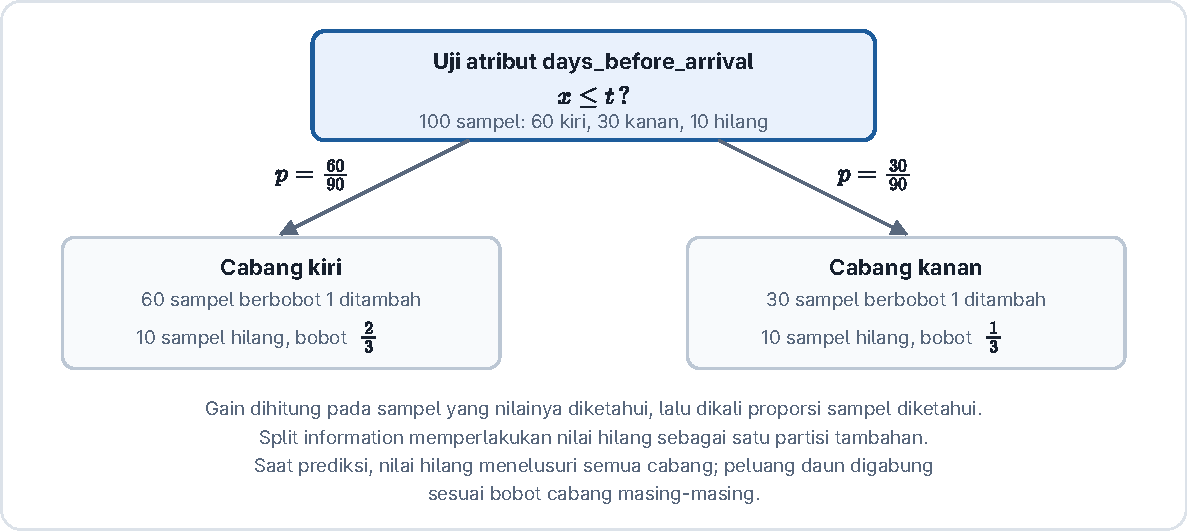
\includegraphics[width=0.82\textwidth]{diagram/dtree.pdf}
    \caption{Distribusi bobot pecahan untuk sampel bernilai hilang pada C4.5.}
    \label{fig:teori-dtree}
\end{figure}

\subsubsection{\textit{Overfitting} dan Pemangkasan}
Pohon yang dibiarkan tumbuh hingga murni cenderung \textit{overfit}, karena daun-daun kecil mencerminkan derau. Pertumbuhan dapat dihentikan lebih awal (\textit{pre-pruning}) melalui batas kedalaman, jumlah sampel minimum, atau \textit{gain} minimum. Pohon juga dapat dipangkas setelah dibangun (\textit{post-pruning}). \textit{Cost-complexity pruning} pada CART meminimalkan
\begin{equation}
    R_\alpha(T)=R(T)+\alpha\,|\widetilde{T}|,
    \label{eq:ccp}
\end{equation}
dengan $R(T)$ galat klasifikasi pohon, $|\widetilde{T}|$ jumlah daun, dan $\alpha\geq0$ harga setiap daun tambahan. Subpohon diganti daun apabila galatnya sebagai daun ditambah $\alpha$ tidak lebih besar daripada jumlah biaya subpohon tersebut. Nilai $\alpha$ dipilih melalui validasi silang.

\subsection{\textit{Logistic Regression}}
\textit{Logistic regression} memodelkan peluang kelas positif dengan fungsi sigmoid dari kombinasi linear fitur:
\begin{equation}
    \hat{p}(\mathbf{x})=\sigma(z)=\frac{1}{1+e^{-z}},\qquad z=\mathbf{w}^\top\mathbf{x}+b.
    \label{eq:sigmoid}
\end{equation}
Batas keputusan $\hat{p}=0{,}5$ setara dengan $z=0$, sehingga model ini menghasilkan hyperplane linear di ruang fitur. Parameter diperoleh dengan memaksimalkan \textit{likelihood}, atau secara setara meminimalkan rata-rata \textit{log-loss} (\textit{binary cross-entropy}):
\begin{equation}
    \mathcal{L}(\mathbf{w},b)=-\frac{1}{n}\sum_{i=1}^{n}\Big[y_i\log\hat{p}_i+(1-y_i)\log(1-\hat{p}_i)\Big].
    \label{eq:logloss}
\end{equation}
Fungsi ini konveks, dan gradiennya berbentuk sederhana:
\begin{equation}
    \nabla_{\mathbf{w}}\mathcal{L}=\frac{1}{n}\sum_{i=1}^{n}(\hat{p}_i-y_i)\,\mathbf{x}_i,\qquad
    \frac{\partial\mathcal{L}}{\partial b}=\frac{1}{n}\sum_{i=1}^{n}(\hat{p}_i-y_i).
    \label{eq:lr-grad}
\end{equation}
\textit{Gradient descent} memperbarui parameter dengan $\mathbf{w}\leftarrow\mathbf{w}-\eta\nabla_{\mathbf{w}}\mathcal{L}$ dengan laju belajar $\eta$. Varian \textit{stochastic} atau \textit{mini-batch} menghitung gradien dari sebagian data pada setiap langkah sehingga pembaruan lebih sering dilakukan. Dalam formulasi \textit{gradient ascent}, kuliah memaksimalkan \textit{log-likelihood}. Kedua formulasi menghasilkan pembaruan yang sama dengan tanda berlawanan.

\subsubsection{Regularisasi}
Regularisasi menambahkan penalti $R(\mathbf{w})$ ke fungsi tujuan, $J=\mathcal{L}+R(\mathbf{w})$, untuk mengendalikan besar bobot dan mengurangi \textit{overfitting}. Bias $b$ umumnya tidak diregularisasi. Tiga bentuk penalti yang diminta adalah
\begin{equation}
    R_{L1}=\alpha\|\mathbf{w}\|_1,\qquad
    R_{L2}=\frac{\alpha}{2}\|\mathbf{w}\|_2^2,\qquad
    R_{EN}=\alpha\left(\rho\|\mathbf{w}\|_1+\frac{1-\rho}{2}\|\mathbf{w}\|_2^2\right),
    \label{eq:reg}
\end{equation}
dengan $\rho$ porsi L1 pada Elastic Net. Penalti L2 (\textit{ridge}) mengecilkan seluruh bobot secara proporsional tanpa membuatnya tepat nol. Penalti L1 (\textit{lasso}) mendorong sebagian bobot menjadi tepat nol sehingga sekaligus melakukan seleksi fitur. Elastic Net menggabungkan keduanya, sehingga tetap menghasilkan bobot jarang tetapi lebih stabil ketika fitur saling berkorelasi. Gambar~\ref{fig:teori-lr} menunjukkan alasan geometrisnya. Kontur \textit{loss} lebih mungkin menyentuh daerah L1 pada sudutnya, yaitu titik dengan salah satu bobot bernilai nol.

Penalti L1 tidak terdiferensialkan di nol. Salah satu cara menanganinya adalah \textit{proximal gradient}. Pada metode ini, langkah gradien dilakukan pada bagian yang mulus, lalu bobot dilewatkan ke operator \textit{soft-threshold}
\begin{equation}
    \mathrm{prox}_{\eta\lambda}(w)=\mathrm{sign}(w)\max(|w|-\eta\lambda,\,0).
    \label{eq:soft-threshold}
\end{equation}
Operator ini menggeser bobot ke arah nol sebesar $\eta\lambda$ dan menetapkannya tepat nol apabila besarnya lebih kecil daripada ambang tersebut.

\begin{figure}[htbp]
    \centering
    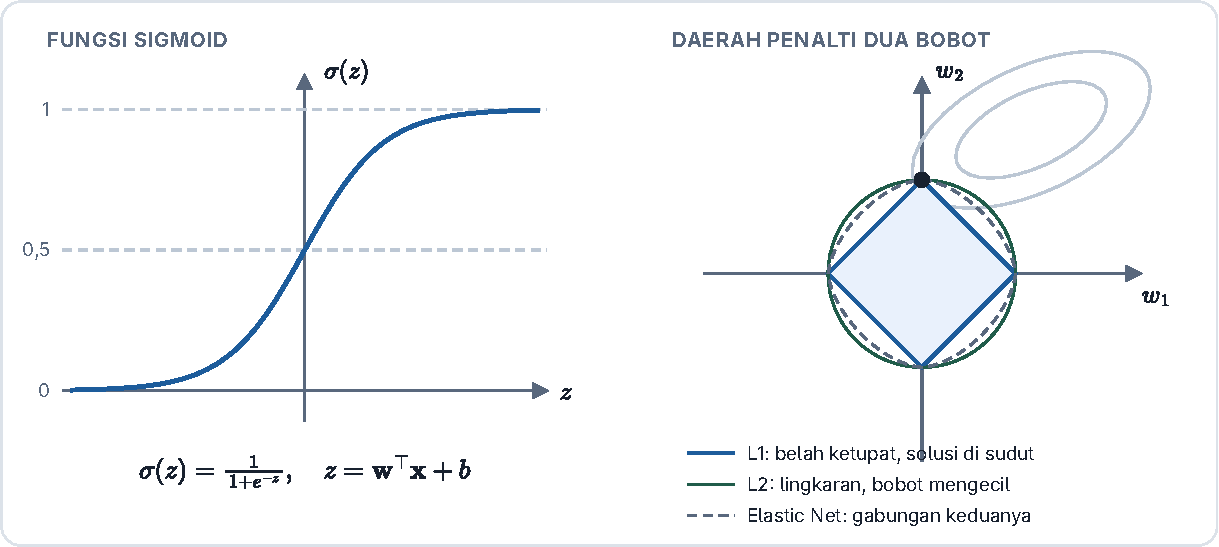
\includegraphics[width=0.92\textwidth]{diagram/logreg.pdf}
    \caption{Fungsi sigmoid (kiri) serta daerah batasan penalti L1, L2, dan Elastic Net pada dua bobot beserta kontur \textit{loss} (kanan).}
    \label{fig:teori-lr}
\end{figure}

\subsection{\textit{Support Vector Machine}}
\textit{Support Vector Machine} (SVM) mencari hyperplane $\mathbf{w}^\top\mathbf{x}+b=0$ yang memisahkan dua kelas dengan margin terbesar. Dengan label $y_i\in\{-1,+1\}$, lebar margin adalah $2/\|\mathbf{w}\|$, sehingga pada data yang terpisah linear persoalannya adalah meminimalkan $\frac{1}{2}\|\mathbf{w}\|^2$ dengan syarat $y_i(\mathbf{w}^\top\mathbf{x}_i+b)\geq1$. Data nyata jarang terpisah sempurna, sehingga \textit{soft-margin} SVM menambahkan variabel \textit{slack} $\xi_i\geq0$:
\begin{equation}
    \min_{\mathbf{w},b,\boldsymbol{\xi}}\ \frac{1}{2}\|\mathbf{w}\|^2+C\sum_{i=1}^{n}\xi_i
    \quad\text{dengan}\quad y_i(\mathbf{w}^\top\mathbf{x}_i+b)\geq1-\xi_i.
    \label{eq:svm-primal}
\end{equation}
Parameter $C$ mengatur kompromi antara margin lebar dan banyaknya pelanggaran. Bentuk dual persoalan ini adalah
\begin{equation}
    \max_{\boldsymbol{\alpha}}\ \sum_{i}\alpha_i-\frac{1}{2}\sum_{i,j}\alpha_i\alpha_j y_i y_j K(\mathbf{x}_i,\mathbf{x}_j)
    \quad\text{dengan}\quad 0\leq\alpha_i\leq C,\ \sum_i\alpha_i y_i=0,
    \label{eq:svm-dual}
\end{equation}
dan fungsi keputusan $f(\mathbf{x})=\sum_{i}\alpha_i y_i K(\mathbf{x}_i,\mathbf{x})+b$. Hanya sampel dengan $\alpha_i>0$ yang memengaruhi $f$. Sampel tersebut disebut \textit{support vector} dan berada pada atau di dalam margin. Gambar~\ref{fig:teori-svm} merangkum konsep margin dan kernel.

\begin{figure}[htbp]
    \centering
    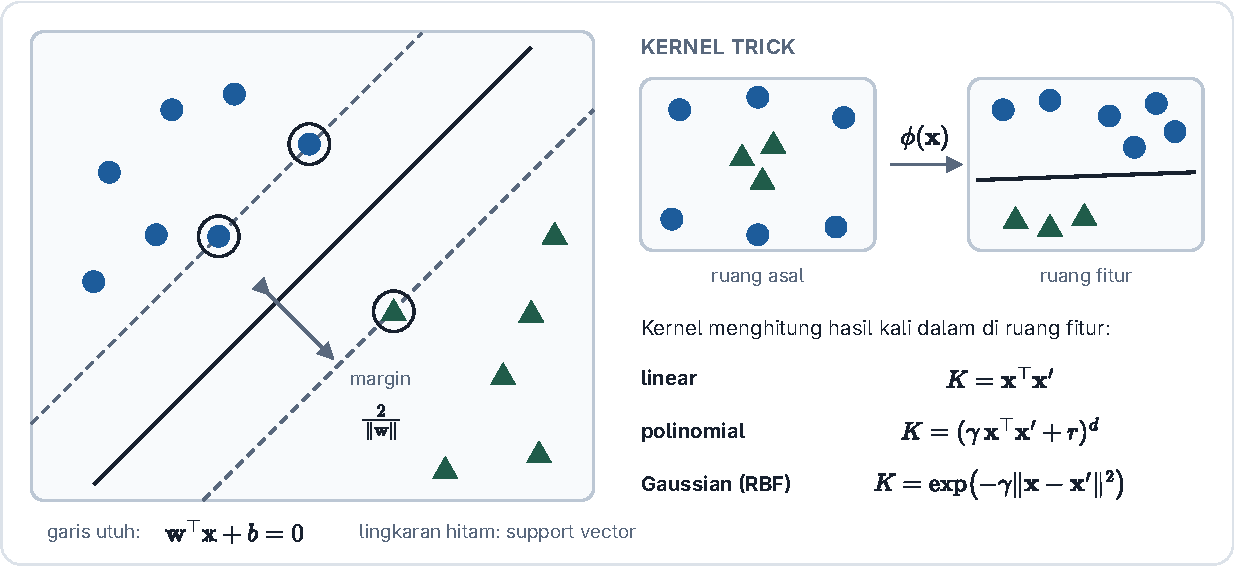
\includegraphics[width=0.95\textwidth]{diagram/svm.pdf}
    \caption{Hyperplane pemisah, margin, dan \textit{support vector} (kiri) serta pemetaan kernel yang membuat data tidak terpisah linear menjadi terpisah di ruang fitur (kanan).}
    \label{fig:teori-svm}
\end{figure}

\subsubsection{Kernel}
Bentuk dual hanya memerlukan hasil kali dalam antarsampel. Fungsi kernel $K(\mathbf{x},\mathbf{x}')=\phi(\mathbf{x})^\top\phi(\mathbf{x}')$ menghitung hasil kali dalam di ruang fitur berdimensi tinggi tanpa membentuk $\phi$ secara eksplisit. Teknik ini disebut \textit{kernel trick}. Tiga kernel yang diminta adalah
\begin{equation}
    K_{\text{lin}}=\mathbf{x}^\top\mathbf{x}',\qquad
    K_{\text{poly}}=(\gamma\,\mathbf{x}^\top\mathbf{x}'+r)^d,\qquad
    K_{\text{RBF}}=\exp\!\left(-\gamma\|\mathbf{x}-\mathbf{x}'\|^2\right).
    \label{eq:kernels}
\end{equation}
Kernel Gaussian (RBF) setara dengan ruang fitur berdimensi tak hingga. Nilai $\gamma$ yang besar membuat pengaruh setiap \textit{support vector} sangat lokal sehingga batas keputusan berliku, sedangkan $\gamma$ kecil menghasilkan batas yang lebih halus.

\subsubsection{\textit{Sequential Minimal Optimization} dan Kalibrasi Peluang}
\textit{Sequential Minimal Optimization} (SMO) menyelesaikan Persamaan~\ref{eq:svm-dual} dengan memperbarui dua pengali $\alpha_i$ dan $\alpha_j$ sekaligus, karena dua variabel adalah jumlah terkecil yang dapat diubah tanpa melanggar syarat $\sum_i\alpha_i y_i=0$. Subpersoalan dua variabel memiliki solusi analitik, lalu hasilnya dipotong ke kotak $[0,C]$. Keerthi dkk. memilih pasangan yang paling melanggar kondisi Karush--Kuhn--Tucker (\textit{maximal violating pair}). Selisih skor pasangan tersebut sekaligus menjadi kriteria berhenti, yaitu optimasi selesai bila selisihnya lebih kecil daripada toleransi. Fan, Chen, dan Lin memperbaiki pemilihan ini dengan informasi orde kedua. Indeks $i$ tetap dipilih sebagai pelanggar terbesar, tetapi $j$ dipilih dari kandidat yang melanggar bersama $i$ dengan meminimalkan $-b_{ij}^2/a_{ij}$. Besaran $b_{ij}$ adalah selisih skor kedua indeks dan $a_{ij}=K_{ii}+K_{jj}-2K_{ij}$, sehingga $-b_{ij}^2/a_{ij}$ adalah penurunan objektif dual bila hanya pasangan tersebut yang diperbarui. Pasangan yang dipilih dengan cara ini menurunkan objektif lebih banyak pada setiap iterasi.

Keluaran SVM berupa margin $f(\mathbf{x})$, bukan peluang. \textit{Platt scaling} memetakan margin ke peluang dengan $P(y=1\mid f)=1/(1+\exp(Af+B))$. Parameter $A$ dan $B$ diestimasi dengan meminimalkan \textit{log-loss} pada data yang tidak dipakai melatih SVM, dengan target yang dihaluskan agar tidak terjadi \textit{overfitting}.

\subsection{\textit{Bayesian Network} dan \textit{Naive Bayes}}
\textit{Bayesian network} adalah graf berarah tak bersiklus yang simpulnya merupakan variabel acak dan busurnya menyatakan ketergantungan langsung. Distribusi gabungan diuraikan menjadi hasil kali peluang bersyarat setiap simpul terhadap induknya, $P(X_1,\dots,X_n)=\prod_i P(X_i\mid\mathrm{Parents}(X_i))$.

\textit{Naive Bayes} adalah \textit{Bayesian network} paling sederhana untuk klasifikasi. Simpul kelas $C$ menjadi satu-satunya induk bagi setiap fitur, dan tidak ada busur antarfitur, sebagaimana diperlihatkan Gambar~\ref{fig:teori-nb}. Struktur ini menyatakan asumsi bahwa fitur saling bebas bersyarat bila kelas diketahui. Dengan teorema Bayes, peluang posterior menjadi
\begin{equation}
    P(C=c\mid x_1,\dots,x_m)=\frac{P(C=c)\prod_{j=1}^{m}P(x_j\mid C=c)}{\sum_{c'}P(C=c')\prod_{j=1}^{m}P(x_j\mid C=c')}.
    \label{eq:nb}
\end{equation}
Prior dan \textit{likelihood} diperkirakan dari frekuensi pada data latih. Agar kategori yang tidak pernah muncul bersama suatu kelas tidak menghasilkan peluang nol, digunakan \textit{Laplace smoothing}:
\begin{equation}
    \hat{P}(x_j=v\mid C=c)=\frac{N_{c,v}+\alpha}{N_c+\alpha\,|V_j|},
    \label{eq:laplace}
\end{equation}
dengan $|V_j|$ banyaknya nilai fitur $j$ dan $\alpha>0$, umumnya $\alpha=1$.

Fitur numerik dapat dimodelkan dengan distribusi Gaussian atau didiskretisasi ke dalam interval. Diskretisasi berbasis kuantil menghasilkan interval dengan jumlah sampel kira-kira sama tanpa melihat label. Sebaliknya, diskretisasi MDL dari Fayyad dan Irani memakai label. Ambang dipilih secara rekursif pada titik yang meminimalkan entropi kelas berbobot, dan sebuah potongan hanya diterima bila
\begin{equation}
    \begin{aligned}
    \mathrm{Gain}(A,T;S)&>\frac{\log_2(N-1)}{N}+\frac{\Delta(A,T;S)}{N},\\
    \Delta(A,T;S)&=\log_2(3^k-2)-\bigl[k\,H(S)-k_1H(S_1)-k_2H(S_2)\bigr],
    \end{aligned}
    \label{eq:fayyad}
\end{equation}
dengan $N$ jumlah sampel pada interval, $k$, $k_1$, dan $k_2$ banyaknya kelas yang muncul pada $S$, $S_1$, dan $S_2$. Jumlah interval tidak ditentukan di depan, sehingga fitur yang tidak informatif dapat tidak dipotong sama sekali.

Hasil kali banyak peluang kecil dapat mengalami \textit{underflow}. Karena itu perhitungan dilakukan dalam ruang logaritma, dan normalisasi memakai \textit{log-sum-exp}, $\log\sum_c e^{s_c}=s^*+\log\sum_c e^{s_c-s^*}$ dengan $s^*=\max_c s_c$. Struktur yang lebih kaya, seperti \textit{Tree Augmented Naive Bayes}, menambahkan busur antarfitur untuk melonggarkan asumsi kebebasan.

\begin{figure}[htbp]
    \centering
    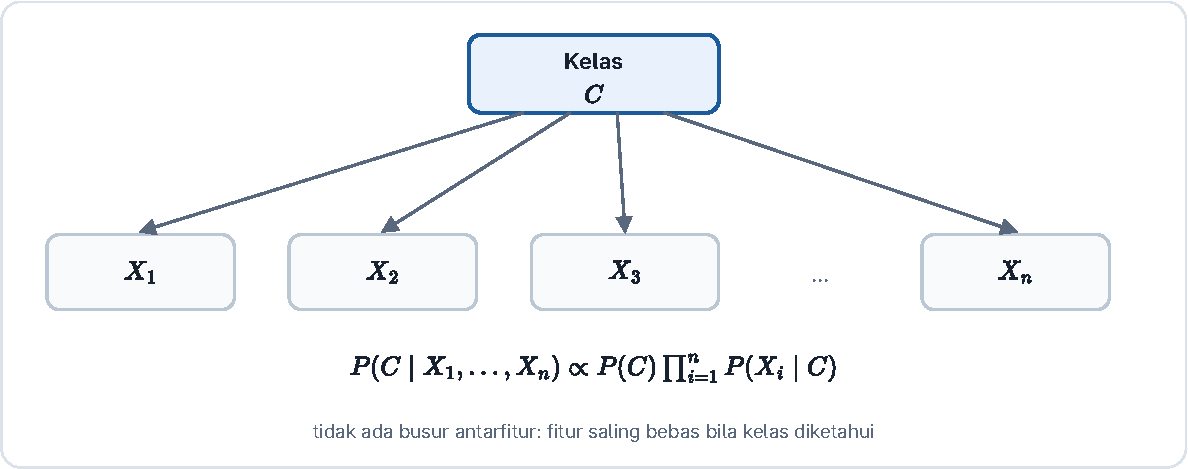
\includegraphics[width=0.78\textwidth]{diagram/naive_bayes.pdf}
    \caption{Struktur \textit{Naive Bayes} sebagai \textit{Bayesian network}.}
    \label{fig:teori-nb}
\end{figure}

\subsection{Validasi Model dan Metrik Evaluasi}
\textit{Train-test split} membagi data berlabel menjadi bagian latih dan validasi. Pembagian berstrata (\textit{stratified}) menjaga proporsi kelas tetap sama pada kedua bagian, yang penting ketika kelas tidak seimbang. \textit{k-fold cross-validation} membagi data menjadi $k$ lipatan. Setiap lipatan bergiliran menjadi validasi sementara $k-1$ lipatan lainnya menjadi data latih, lalu skor dirata-rata. Estimasi ini lebih stabil daripada satu pembagian, dengan syarat seluruh tahap persiapan data di-\textit{fit} ulang di dalam setiap lipatan. Skemanya ditunjukkan Gambar~\ref{fig:teori-kfold}.

\begin{figure}[htbp]
    \centering
    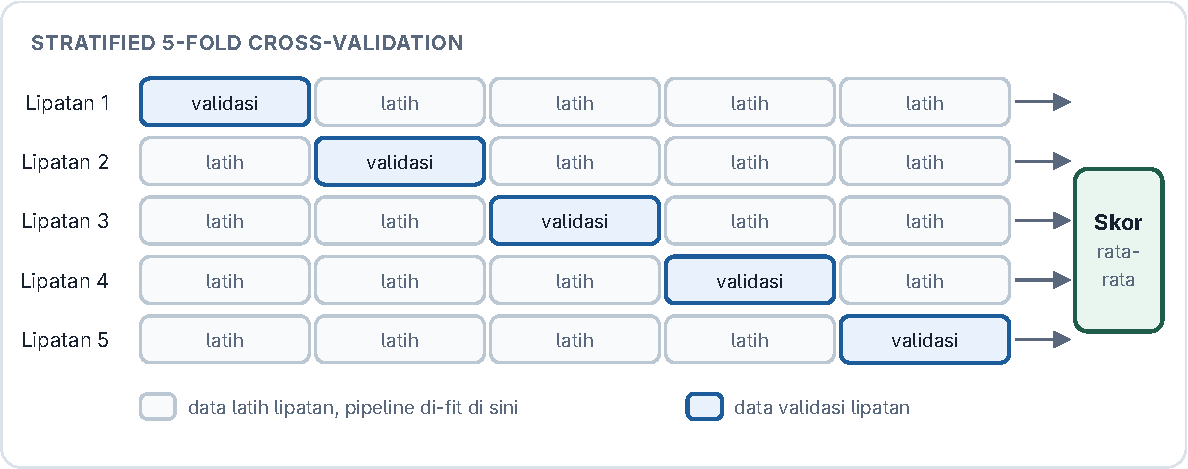
\includegraphics[width=0.8\textwidth]{diagram/kfold.pdf}
    \caption{\textit{Stratified 5-fold cross-validation}.}
    \label{fig:teori-kfold}
\end{figure}

Hasil klasifikasi biner dirangkum dalam \textit{confusion matrix} yang memuat \textit{true positive} (TP), \textit{true negative} (TN), \textit{false positive} (FP), dan \textit{false negative} (FN). Metrik yang digunakan adalah
\begin{equation}
    \mathrm{Acc}=\frac{TP+TN}{TP+TN+FP+FN},\quad
    \mathrm{Prec}=\frac{TP}{TP+FP},\quad
    \mathrm{Rec}=\frac{TP}{TP+FN},\quad
    F_1=\frac{2\,\mathrm{Prec}\cdot\mathrm{Rec}}{\mathrm{Prec}+\mathrm{Rec}}.
    \label{eq:metrics}
\end{equation}
Akurasi mudah ditafsirkan, tetapi pada data tidak seimbang model yang selalu menebak kelas mayoritas pun dapat memperoleh akurasi cukup tinggi. Presisi menjawab berapa bagian prediksi batal yang benar, sedangkan \textit{recall} menjawab berapa bagian pembatalan yang terdeteksi. ROC-AUC adalah luas di bawah kurva \textit{true positive rate} terhadap \textit{false positive rate} untuk seluruh ambang. Nilainya sama dengan peluang model memberi skor lebih tinggi kepada sampel positif acak daripada sampel negatif acak, sehingga dapat dihitung melalui statistik peringkat Mann--Whitney tanpa menetapkan ambang.

\subsection{\textit{Cost-Sensitive Classification}}\label{sec:teori-cost}
Pada banyak persoalan, jenis kesalahan berbeda memiliki biaya berbeda. Misalkan biaya FP adalah $c_{FP}$ dan biaya FN adalah $c_{FN}$. Untuk sampel dengan peluang positif $p$, memprediksi positif memberi biaya harapan $(1-p)\,c_{FP}$, sedangkan memprediksi negatif memberi $p\,c_{FN}$. Prediksi positif lebih murah bila $(1-p)c_{FP}<p\,c_{FN}$, sehingga ambang keputusan optimum adalah
\begin{equation}
    \tau^*=\frac{c_{FP}}{c_{FP}+c_{FN}}.
    \label{eq:cost-threshold}
\end{equation}
Dengan $c_{FP}=2$ dan $c_{FN}=1$, diperoleh $\tau^*=2/3$. Aturan ini hanya tepat jika peluang model terkalibrasi. Bila tidak, ambang dapat dicari secara empiris dengan meminimalkan biaya total $2\,FP+FN$ pada data validasi.
 Gambar~\ref{fig:teori-confusion} menunjukkan letak biaya pada \textit{confusion matrix}.

\begin{figure}[htbp]
    \centering
    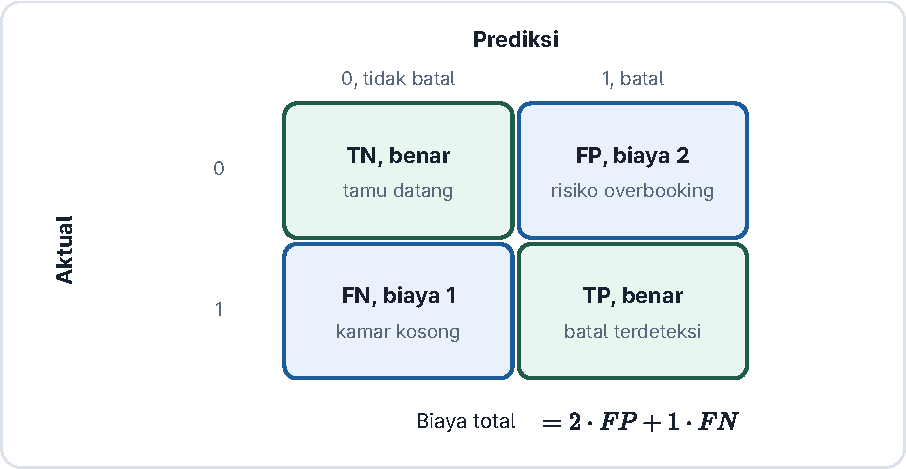
\includegraphics[width=0.6\textwidth]{diagram/confusion.pdf}
    \caption{\textit{Confusion matrix} dan biaya kesalahan pada persoalan pembatalan pemesanan.}
    \label{fig:teori-confusion}
\end{figure}

\subsection{Algoritma Optimasi Model}
Bagian ini merangkum algoritma optimasi di luar materi kelas yang dipakai untuk meningkatkan kinerja model.
\begin{enumerate}
    \setlength{\itemsep}{0pt}
    \item \textbf{FISTA}\\
    \textit{Gradient descent} proksimal (ISTA) memiliki laju konvergensi objektif $O(1/k)$. FISTA menambahkan momentum Nesterov. Langkah gradien dan \textit{soft-threshold} dihitung pada titik ekstrapolasi $\mathbf{z}_k=\boldsymbol{\theta}_k+\frac{t_k-1}{t_{k+1}}(\boldsymbol{\theta}_k-\boldsymbol{\theta}_{k-1})$ dengan $t_{k+1}=\bigl(1+\sqrt{1+4t_k^2}\bigr)/2$, sehingga laju konvergensinya menjadi $O(1/k^2)$. Ukuran langkah $1/L$ diturunkan dari konstanta Lipschitz gradien \textit{log-loss}, yaitu $L=\lambda_{\max}(\mathbf{X}^\top\mathbf{X}/n)/4$ ditambah koefisien L2. Karena tetap memakai operator proksimal, FISTA berlaku untuk L1 dan Elastic Net.
    \item \textbf{Adam}\\
    Adam menyimpan rata-rata bergerak gradien $m_t=\beta_1 m_{t-1}+(1-\beta_1)g_t$ dan kuadrat gradien $v_t=\beta_2 v_{t-1}+(1-\beta_2)g_t^2$. Setelah koreksi bias $\hat{m}_t=m_t/(1-\beta_1^t)$ dan $\hat{v}_t=v_t/(1-\beta_2^t)$, parameter diperbarui dengan $\theta\leftarrow\theta-\eta\,\hat{m}_t/(\sqrt{\hat{v}_t}+\epsilon)$. Setiap parameter memperoleh ukuran langkah sendiri, sehingga parameter dengan gradien kecil tetap bergerak cukup jauh. Adam dirancang untuk fungsi tujuan yang mulus, sehingga pada implementasi kelompok Adam hanya dipakai untuk penalti L2 atau tanpa penalti.
    \item \textbf{\textit{Cost-complexity pruning}}\\
    Pohon penuh dipangkas dengan meminimalkan Persamaan~\ref{eq:ccp}. Nilai $\alpha$ yang lebih besar menghasilkan pohon yang lebih kecil, dan $\alpha$ terbaik dipilih dengan validasi silang.
    \item \textbf{\textit{Random search}}\\
    Konfigurasi \textit{hyperparameter} diambil secara acak dari ruang pencarian dan dinilai dengan validasi silang. Pada ruang berdimensi tinggi yang hanya sebagian dimensinya berpengaruh, \textit{random search} lebih efisien daripada \textit{grid search} dengan anggaran percobaan yang sama.
    \item \textbf{Penalti MDL untuk atribut kontinu}\\
    Atribut kontinu dengan $N$ nilai berbeda memiliki $N-1$ kandidat ambang, sehingga peluang menemukan ambang yang tampak baik secara kebetulan meningkat. Quinlan mengusulkan pengurangan \textit{information gain} sebesar $\log_2(N-1)/|D|$, dengan $|D|$ jumlah sampel pada simpul. Penalti ini mengikuti prinsip \textit{minimum description length} (MDL), yaitu biaya untuk menyandikan pilihan ambang, dan atribut yang \textit{gain}-nya tidak positif setelah dikurangi penalti tidak dipakai.
    \item \textbf{Diskretisasi MDL pada \textit{Naive Bayes}}\\
    Interval kuantil diganti dengan ambang Fayyad--Irani pada Persamaan~\ref{eq:fayyad}. Ambang ditentukan oleh hubungan fitur dengan label, sehingga fitur yang jarang bernilai positif tetap dapat memiliki potongan.
    \item \textbf{Seleksi \textit{working set} orde kedua pada SMO}\\
    Indeks kedua pada SMO dipilih dengan kriteria $-b_{ij}^2/a_{ij}$ dari Fan, Chen, dan Lin. Kriteria berhenti tetap celah KKT pasangan pelanggar maksimal, sehingga solusi yang dicapai sama dan yang berubah hanya jumlah iterasi.
\end{enumerate}
